\documentclass[pdflatex,sn-mathphys-num]{sn-jnl}

\usepackage{graphicx}
\usepackage{multirow}
\usepackage{amsmath,amssymb,amsfonts}
\usepackage{amsthm}
\usepackage[title]{appendix}
\usepackage{xcolor}
\usepackage{textcomp}
\usepackage{manyfoot}
\usepackage{booktabs}
\usepackage{algorithm}
\usepackage{algorithmicx}
\usepackage{algpseudocode}
\usepackage{listings}

\graphicspath{{figs/}{./figs/}{./}}
\setkeys{Gin}{draft=false}

\newcommand{\figref}[1]{Figure~\ref{#1}}
\newcommand{\parstart}[2]{#1#2}

\raggedbottom

\AtBeginDocument{%
  \addtolength{\oddsidemargin}{\evensidemargin}%
  \setlength{\oddsidemargin}{0.5\oddsidemargin}%
  \setlength{\evensidemargin}{\oddsidemargin}%
}

\hypersetup{bookmarksdepth=3}

\AtBeginDocument{%
  \let\snOrigThebibliography\thebibliography
  \renewcommand{\thebibliography}[1]{%
    \snOrigThebibliography{#1}\sloppy\hbadness=10000\relax}%
}

\begin{document}

\title[Prompted labels and easy negatives inflate cough detection accuracy]{Prompted
labels and easy negatives inflate cough detection accuracy: a controlled comparison
across three label regimes}

\author[1]{\fnm{Prayag} \sur{Sharma}}\email{prayag.sharma2024@vitstudent.ac.in}

\author*[2]{\fnm{Ravi} \sur{Tiwari}}\email{ravi.tiwari@vit.ac.in}

\affil[1]{\orgdiv{School of Computer Science and Engineering (SCOPE)},
\orgname{Vellore Institute of Technology}, \orgaddress{\city{Chennai},
\state{Tamil Nadu}, \country{India}}}

\affil*[2]{\orgdiv{School of Electronics Engineering (SENSE)},
\orgname{Vellore Institute of Technology}, \orgaddress{\city{Chennai},
\state{Tamil Nadu}, \country{India}}}

\abstract{Reported accuracies for cough detection sit in the high nineties, yet such
models are rarely validated outside their development corpus. The responsible factor has
not been isolated, because label provenance, negative class difficulty and seed variation
ordinarily move together. This study fixes preprocessing, architecture and training
protocol, and varies only label provenance. Three corpora are used, labelled respectively
by a participant's instruction, by another classifier's score, and by a human listener
against an audio ontology. The class prior is matched in all three, partitions are speaker
disjoint wherever an identifier permits, every condition runs under five seeds, and
conditions are compared by a paired test on per recording decisions. Within the prompted
corpus a residual network reaches 98.6 per cent balanced accuracy on held out speakers.
The same weights, applied without retraining to human annotated audio at the same prior,
reach 70.2 per cent: specificity falls to 84.3 per cent and sensitivity to 56.0. The loss
is one of discrimination rather than calibration, the area under the curve falling from
0.998 to 0.749, so moving the threshold recovers little of it. Sneezes are assigned to the
cough class more often than coughs are, locating the failure in a negative class holding
no forced expiration. Wavelet shrinkage does not help, removing a median of 0.67 per cent
of signal power. The classifier labelled corpus cannot be reproduced from the score it
publishes. The external set is small and single source, so the fall is better established
in direction than size.}

\keywords{Audio classification, dataset bias, external validation, label provenance, respiratory
sound analysis, wavelet shrinkage}

\maketitle

\section{Introduction}\label{sec:intro}

\parstart{C}{oughing} is among the few sounds the body produces that carries diagnostic information and
can be recorded without instrumentation, a clinician or a visit. That combination is what
has made automatic cough analysis attractive: a microphone is already in every pocket, and
a cough is loud, brief and distinctive. Almost every application proposed for it, from
monitoring the progression of a chronic respiratory condition to triaging an infectious
one, rests on a step that is rarely the subject of the paper that uses it. Before anything
can be inferred from a cough, the cough has to be found. Detection is the foundation, and
the quality of that foundation sets a ceiling on everything built above it.

The reported accuracy of that foundational step is, on its face, settled. Work on cough
and respiratory audio routinely reports accuracies in the high nineties, on architectures
ranging from purpose built convolutional networks to transfer learning from image
classification~\cite{imran2020, laguarta2020, pahar2021}. A reader encountering these
figures would reasonably conclude that cough detection is solved and that attention
belongs further downstream.

A sequence of independent audits has since established that this conclusion does not
follow from the evidence offered for it. Reviews of machine learning applied to
respiratory audio during the pandemic found that the overwhelming majority of published
models carried a high risk of bias and that almost none were validated on data from a
source other than the one they were developed on~\cite{roberts2021}. More specifically,
models that appeared to detect disease were shown to be reading confounds instead: the
recording device, the collection site, the prompt a participant was reading, or simply the
identity of the speaker, any of which can separate the classes when the classes were not
collected under matched conditions~\cite{han2022, coppock2024}. Where an external test set
was eventually applied, performance fell to near chance~\cite{xia2021, zhou2021}. The
pattern across these audits is consistent, and it is not that the models were badly
trained. It is that the evaluations measured something other than what they were taken to
measure.

This leaves a specific and answerable question, and it is the one this work addresses. The
audits identified that single corpus evaluation inflates performance, but they did not
isolate which part of the evaluation is responsible, because in the studies they examined
several candidate causes vary together. Three in particular are routinely conflated. The
first is the provenance of the label: a recording may be called a cough because a
participant was told to cough, because a person listened and judged that a cough was
present, or because another classifier assigned it a score above a threshold. These are
treated throughout the literature as interchangeable sources of ground truth, and they are
not equivalent claims. The second is the composition of the negative class. Separating
coughing from a sustained vowel is a different problem from separating it from breathing,
sneezing, gasping and laughter, and a corpus whose negatives happen to be easy will
reward a detector that has learned very little. The third is run to run variation.
Differences well under one accuracy point are reported as findings in this area without
any estimate of the spread across random seeds, which is the quantity that determines
whether such a difference can be claimed at all.

The present work holds the architecture, the preprocessing and the training protocol fixed
and varies these three factors deliberately. Three corpora are used, chosen so that each
represents one label regime: prompt derived labels from Coswara~\cite{coswara2020}, human
annotated labels from the exhaustively verified evaluation split of
FSD50K~\cite{fsd50k2022}, and classifier derived labels from the \texttt{cough\_detected}
score shipped with COUGHVID~\cite{coughvid2021}. The class prior is matched across all
three by construction, so a change in performance between regimes cannot be attributed to
a change in class balance. Partitions over the prompt derived corpus are built over
participants rather than recordings, so no speaker appears on both sides of a split.
Every condition is run under five random seeds, and every comparison is tested on paired
per recording decisions rather than on summary accuracies.

The specific contributions are the following.

\begin{itemize}
\item A controlled comparison of the three label regimes under one fixed pipeline, in
      which label provenance is the variable and class prior, preprocessing, architecture
      and training protocol are held constant. This isolates a factor that the existing
      audits identified but did not separate from the others varying alongside it.

\item A quantification of how far single corpus accuracy overstates detection. Under an
      identical input condition, ResNet18 reaches $98.6$ per cent balanced accuracy on
      held out speakers from the prompted corpus and $70.2$ per cent on the human
      annotated split, and the fall is asymmetric in a way that a single accuracy figure
      conceals: specificity declines from $99.5$ to $84.3$ per cent while sensitivity
      collapses from $97.7$ to $56.0$. A detector that appears to be near perfect misses
      close to half of all coughs once the negatives are confusable and the labels come
      from a person. The loss is shown to lie in discrimination rather than in
      calibration, which closes off the cheapest remedy: the area under the curve falls
      from $0.998$ to $0.749$, and moving the decision threshold to the best position for
      the external set recovers only $1.7$ points.

\item An account of what the detectors confuse, obtained from the annotated classes of
      the external negatives. The false positives are concentrated rather than diffuse,
      and they fall on the other forced expirations: clips labelled as sneezes are
      assigned to the cough class in $67.8$ per cent of decisions, a higher rate than the
      same models achieve on clips that are genuinely coughs. The negative class of the
      prompted corpus contains no forced expiration, so the distinction was never one the
      models were required to learn.

\item An assessment of wavelet shrinkage as a preprocessing step under a protocol able to
      detect an effect of the size being claimed for it. Measured against the spread across
      seeds, the gain does not survive: the largest improvement observed anywhere is
      $2.73$ accuracy points, with a spread of $3.54$ points across the seeds it
      is averaged over. The mechanism is measured rather than inferred: on
      recordings of this quality the universal threshold removes a median of
      $0.67$ per cent of the signal power, so the two conditions it produces are
      very nearly the same images.

\item A reproducibility finding about the classifier derived corpus. The recording
      selection used by the work this study extends cannot be reproduced from the corpus as
      published, for an arithmetic reason that is demonstrated rather than asserted, and
      the expert annotated subset cannot be used to estimate the corpus label error rate
      because it is not a random sample of the corpus.

\end{itemize}

The computational conditions are stated in enough detail to be acted upon rather than
merely reproduced, and Section~\ref{sec:setup-train} records a measured account of one
failure mode that produces no error and no warning while costing a factor of $6.4$ in
training throughput, together with the measurement that distinguishes its cause from the
plausible alternative.

Nothing in what follows should be read as a claim that cough detection is unachievable, or
that the architectures examined here are inadequate to it. The networks fit the prompted
corpus almost perfectly, and they do so from a speaker disjoint partition, which rules out
the simplest explanation for a high score. The claim is narrower and, for anyone intending
to build on such a result, more consequential: the number obtained that way does not
transfer, the direction in which it fails is predictable, and the experiment needed to
discover this costs far less than the experiment that assumes otherwise.

The remainder of the paper is organised as follows.
Section~\ref{sec:related} reviews classifiers built on cough audio, what has since been
established about how they were evaluated, and the evidence offered for denoising as a
preprocessing step. Section~\ref{sec:design} sets out the pipeline, taking the wavelet
shrinkage, the spectrogram and the networks in the order the signal meets them.
Section~\ref{sec:setup} describes the corpora and their label regimes, the partitioning,
the training protocol and the statistical procedure. Section~\ref{sec:results} reports the
grid, the external evaluation and the comparison across regimes.
Section~\ref{sec:discussion} draws out what follows for how detectors of this kind should
be evaluated and what the corpora would need to contain.
Section~\ref{sec:conclusion} states what the results support and what they do not.

\section{Related work and its limitations}\label{sec:related}

The literature this work sits in divides into four strands, and the gap it addresses lies
between them. Section~\ref{sec:rel-class} covers classifiers built on cough and
respiratory audio, Section~\ref{sec:rel-eval} covers what has since been established
about how their performance was measured, Section~\ref{sec:rel-neg} covers the
composition of the negative class and what it determines, and
Section~\ref{sec:rel-denoise} covers denoising as a preprocessing step and states what
the present work supplies that none of these provide.

\subsection{Classifiers on cough and respiratory audio}\label{sec:rel-class}

Interest in classifying respiratory audio grew sharply during the COVID-19 pandemic, and
the resulting body of work established the pipeline this paper studies. An early mobile
system passed three second cough recordings to a cloud classifier and returned a
screening result, reporting that it was a screening aid rather than a clinical grade
test~\cite{imran2020}. A convolutional model trained on recordings collected through a web
form reported $98.5$ per cent sensitivity at $94.2$ per cent specificity against official
test results~\cite{laguarta2020}. Working from the Coswara corpus together with a smaller
clinical collection, a comparison of seven classifiers reported area under the curve of
$0.98$ separating positive from healthy coughs, and additionally observed that positive
coughs were some $15$ to $20$ per cent shorter~\cite{pahar2021}.

The supporting corpora were assembled over the same period, and their design decisions
shape what can be asked of them. Coswara records each participant performing a prescribed
sequence of breathing, cough and voice tasks and carries a participant
identifier~\cite{coswara2020}. COUGHVID gathered some $34{,}000$ recordings through a web
form and, because no human could annotate them all, shipped the output of a cough
detector as a per recording score~\cite{coughvid2021}. A larger crowdsourced collection
assembled over $53{,}000$ samples from more than $36{,}000$ participants and published
benchmarks for symptom and condition prediction~\cite{xia2021}. Outside the respiratory
setting, general purpose audio event corpora provide human annotations against a shared
ontology~\cite{gemmeke2017}, and one such corpus had its evaluation split exhaustively
verified by hand~\cite{fsd50k2022}, which is what makes it usable as an independent test
of a detector trained elsewhere.

Within this strand, the specific pipeline of interest is the one that converts a
recording into a spectrogram image and hands it to a convolutional network pretrained on
photographs. That approach reported $98.18$ per cent accuracy on a mel spectrogram
representation of cough audio~\cite{zhou2021}, and variants of it supply the architectures
used here~\cite{he2016,sandler2018,huang2017}. Detection of the event itself continues to be
pursued in this form and in others, with recent work reporting neural cough
counting from audio~\cite{feng2024}, detection from acceleration signals in
place of sound~\cite{sanchezmorillo2024}, and screening pipelines built on
cough audio for {COVID-19}~\cite{ayappan2025}.

\subsection{How the reported performance was measured}\label{sec:rel-eval}

The second strand is the subsequent examination of those results, and it is the reason
this paper is organised around measurement rather than around a new architecture. A
systematic review of machine learning applied to COVID-19 imaging screened $2{,}212$
studies, retained $62$ after quality assessment, and concluded that none of the models it
examined was of potential clinical use, attributing this to methodological flaws and
underlying biases rather than to insufficient model
capacity~\cite{roberts2021}. The same pattern was then demonstrated directly on audio. In
a study of $67{,}842$ participants, classifiers that reached $0.846$ area under the curve
unadjusted fell to $0.619$ once confounders including self-reported symptoms were matched,
and were outperformed by predictions from self-reported symptoms
alone~\cite{coppock2024}. A matched analysis on crowdsourced respiratory audio reported
$0.71$ area under the curve for a model evaluated on participant independent partitions,
against up to $0.90$ for the same material under a less careful evaluation
strategy~\cite{han2022}.

Three specific weaknesses recur, and each is addressed by a part of the present design.
The first is the split. Where a partition is made over recordings rather than
contributors, a contributor can appear on both sides of it. One study reports both
variants and so quantifies the cost: $98.18$ per cent under a random split against
$95.18$ per cent when test coughs came from recordings unseen in training, a gap it
presents without comment~\cite{zhou2021}. The second is what the learned representation
actually encodes. A recent cross-dataset evaluation of cough models found that
performance moderate within a corpus falls below $0.6$ area under the curve on
independent data, and that the representations cluster by recording device and corpus
rather than by the condition being detected~\cite{zhang2026}; two of its authors are also
authors of COUGHVID~\cite{coughvid2021}. The third is the absence of any estimate of run
to run variation, which leaves differences of well under one accuracy point reported as
findings with nothing to read them against.

A fourth weakness is specific to corpora whose labels come from a classifier. Where the
label is a thresholded detector score, a model is measured on its agreement with that
detector and not on whether a cough is present, and this distinction is frequently left
implicit. It cannot be resolved by better modelling, only by stating the regime and, where
possible, comparing across regimes.

The practices this strand calls for have begun to appear in the literature it
examines. External validation of cough based screening algorithms on data
collected independently of the development corpus has been reported for
tuberculosis~\cite{zimmer2026}; an evaluation protocol corrected for leakage
has been proposed for respiratory sound classification~\cite{park2026}; a
patient disjoint partition has been applied across two public
databases~\cite{niu2026}; a feature comparison has been published with
reproduction as an explicit objective~\cite{smailov2026}; and a methodological
framework has been assessed on a corpus whose labels were clinically
validated~\cite{aquino2026}. The recording device has likewise been treated as
a distribution shift in its own right rather than as noise~\cite{wu2026}.

\subsection{The negative class and what it determines}\label{sec:rel-neg}

A detector learns the boundary it is asked to draw, and in a two class problem that
boundary is fixed as much by what the negatives contain as by what the positives do. This
is implicit in the corpora rather than discussed in the papers built on them, and it
deserves stating, because the three corpora used here arrive at their negatives in three
quite different ways.

A prompted collection obtains its negatives the same way it obtains its positives, by
asking. Coswara asks participants for breathing, for sustained vowels and for
counting~\cite{coswara2020}, so the negative class is whatever those tasks produce. This
has a property worth keeping, in that both classes then come from the same participant,
the same device and the same session, so a difference between them cannot be an artefact
of channel or speaker. It also has a property worth noticing: not one of those tasks is a
forced expiration. Sneezing, throat clearing, burping and gasping share with coughing the
mechanism that makes it acoustically distinctive, and none of them is present.

A crowdsourced collection takes whatever arrives. The negatives are then as varied as the
contributors, which is a kind of difficulty, but it is unstructured, and the corpus
cannot say which confusions it does or does not cover~\cite{xia2021, coughvid2021}. A
corpus annotated against a general ontology is the only one of the three that can. Because
the ontology names breathing, sneezing, gasping, sighing and laughter as separate
classes~\cite{gemmeke2017}, a negative class can be assembled from them deliberately
rather than accepted as whatever happened to score low on a
detector~\cite{fsd50k2022, vocalsound2022}.

The consequence for evaluation is that a specificity figure is uninterpretable without a
description of what the negatives were. Two detectors reporting the same specificity may
have been tested against entirely different problems, and the one tested against the
easier negatives will appear equal to the other while being substantially worse at the
task either is meant to perform. The cross-dataset evaluation noted above is consistent
with this, in finding that representations cluster by corpus rather than by the condition
being detected~\cite{zhang2026}. What has not been reported, and what
Section~\ref{sec:res-external} supplies, is an attribution of the false positives to the
annotated classes that produced them, which is what identifies the specific confusion a
training corpus failed to teach.

\subsection{Denoising as a preprocessing step}\label{sec:rel-denoise}

The third strand is the preprocessing itself. Wavelet shrinkage has a well established
theory: the universal threshold with soft thresholding comes with an oracle
inequality~\cite{donoho1994}, a level adaptive threshold derived in a Bayesian framework
improves on it for image data~\cite{chang2000}, and an empirical Bayes rule with a mixture
prior estimates the sparsity of each scale from the data rather than assuming
it~\cite{johnstone2005}. All three rest on the same multiresolution
decomposition~\cite{mallat1989}, and the appeal for cough audio is that shrinkage
suppresses broadband noise while preserving transients, which is what a cough is.

What is missing is a comparison that isolates the effect. Where denoising is reported to
help, the denoised and undenoised conditions commonly differ in more than the denoising,
the shrinkage rule is often not named even though the three rules above behave quite
differently, and the comparison is typically between two single runs with no paired test
and no measure of seed variation. The work this paper extends illustrates all three: its
baseline and denoised conditions differ in architecture, in pretraining, in frequency axis
and in sample rate simultaneously, so no cause can be assigned to the difference between
them; its text describes soft thresholding while the routine it calls applies an empirical
Bayes posterior median by default; and its conclusion rests on one run per condition. How much preprocessing is warranted remains open, and a
minimal preprocessing paradigm has recently been argued for detection from
cough audio~\cite{lim2026}.

The present work therefore supplies what this configuration of strands leaves absent: a
denoising comparison under a named shrinkage rule, with the architecture, the frequency
axis, the partition and the training protocol held fixed, on a speaker disjoint partition
in which both classes come from the same participant and session, tested on paired per
recording decisions with a correction for multiple comparisons, repeated across seeds so
that the size of an effect can be read against the variation between runs, and carried
out across three label regimes rather than one. The contribution is the measurement, not
a new architecture.

\section{System design}\label{sec:design}

The pipeline turns a recording into a fixed size image and then classifies that image.
Three choices inside it are the subject of the study, and this section takes them in the
order the signal meets them: Section~\ref{sec:design-denoise} covers the wavelet
denoising applied to the waveform, Section~\ref{sec:design-spectro} covers the
spectrogram that is formed from the result, and Section~\ref{sec:design-nets} covers the
four networks the images are shown to. Everything else about the pipeline is held fixed
across conditions so that a difference in the outcome can be attributed to one of these
three.

\subsection{Wavelet denoising of the waveform}\label{sec:design-denoise}

A crowdsourced recording carries whatever noise the contributor's room and microphone
supplied. Wavelet shrinkage is an established way to suppress such noise while preserving
transients~\cite{donoho1994}, which matters here because a cough is a transient and a
method that smooths it away would destroy the thing being detected.

The waveform $x$ is decomposed to level $J = 6$ with the \texttt{sym4} wavelet using the
discrete wavelet transform, computed by the pyramidal algorithm of
Mallat~\cite{mallat1989}. This yields detail coefficients $d_{j,k}$ at scales
$j = 1, \dots, J$ and a residual approximation. Shrinkage is applied to the detail
coefficients only, and the signal is reconstructed from the shrunk coefficients.

Which shrinkage rule is used is not a detail that can be left implicit, because the
reported effect of denoising depends on it entirely. Three rules appear in this work and
they are distinguished throughout. The universal threshold of Donoho and
Johnstone~\cite{donoho1994}, applied with soft thresholding, sets one threshold for the
whole decomposition from an estimate $\hat{\sigma}$ of the noise level:
\begin{equation}
\lambda_{\mathrm{uni}} = \hat{\sigma}\sqrt{2\ln n},
\qquad
\eta_{\mathrm{soft}}(d) = \operatorname{sgn}(d)\,\max(|d| - \lambda, 0),
\label{eq:visu}
\end{equation}
where $n$ is the number of samples and $\hat{\sigma}$ is taken from the median absolute
deviation of the finest scale coefficients. The level adaptive rule of Chang, Yu and
Vetterli~\cite{chang2000} instead sets a threshold per scale from the ratio of the noise
variance to the estimated signal variance $\hat{\sigma}_{x,j}^{2}$ at that scale:
\begin{equation}
\lambda_{\mathrm{bayes},j} = \frac{\hat{\sigma}^{2}}{\hat{\sigma}_{x,j}},
\qquad
\hat{\sigma}_{x,j}^{2} = \max\!\left(\widehat{\operatorname{var}}(d_{j,\cdot})
  - \hat{\sigma}^{2},\, 0\right).
\label{eq:bayes}
\end{equation}
The third rule is the empirical Bayes procedure of Johnstone and
Silverman~\cite{johnstone2005}, which places a mixture prior on each coefficient,
\begin{equation}
d_{j,k} \sim (1 - w_j)\,\delta_0 + w_j\,\gamma,
\label{eq:eb}
\end{equation}
with $\delta_0$ a point mass at zero, $\gamma$ a heavy tailed density, and the mixing
weight $w_j$ estimated from the coefficients at that scale by marginal maximum
likelihood. The coefficient is then replaced by the median of its posterior.

This matters for interpreting the work being extended. Its implementation calls a
denoising routine without naming a rule, and the default of that routine is the empirical
Bayes procedure of Equation~\ref{eq:eb} with a Cauchy prior and the posterior median,
not the soft thresholding of Equation~\ref{eq:visu}. The denoising reported here
implements Equations~\ref{eq:visu} and~\ref{eq:bayes} directly and states which is in
use. It is therefore a replication under a specified denoiser rather than a reproduction
of that routine, and it is not expected to agree with it coefficient by coefficient. The
alternative, reporting a result under a rule that was never named, is what makes a
denoising comparison impossible to check.

\figref{fig:denoise} shows what the shrinkage removes, for one cough and one
non-cough recording drawn from the classifier derived corpus, the one whose archive is
retained locally after imaging. The left column of the figure is the waveform as
recorded and the right column is the component the shrinkage discarded, drawn on its own
vertical scale because against the signal it is a flat line at zero; the magnification
needed to make it visible is printed on each panel, beside the fraction of signal power
it accounts for. What is removed is a low level broadband residual rather than any part
of the event itself.
Measured across $259$ recordings, the universal threshold removes a median of $0.67$ per
cent of the signal power, with quartiles at $0.08$ and $2.28$ per cent, and the empirical
Bayes rule removes $0.0014$ per cent. \figref{fig:power} gives the distribution over the audit set for both rules.

\begin{figure}[tbp]
\centering
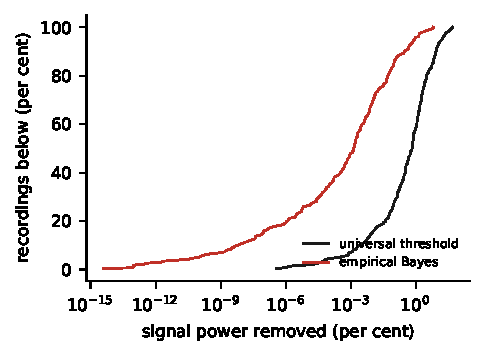
\includegraphics[width=0.98\columnwidth]{shrinkage.pdf}
\caption{Signal power removed by each shrinkage rule, over the audit set.}\label{fig:power}
\end{figure} It is worth establishing this before any result is
reported, because it bounds what the comparison can show. Whatever the shrinkage does to
recordings of this kind, it does very little of it, and the two input conditions that
follow from it are very nearly the same images.

\begin{figure*}[tbp]
\centering
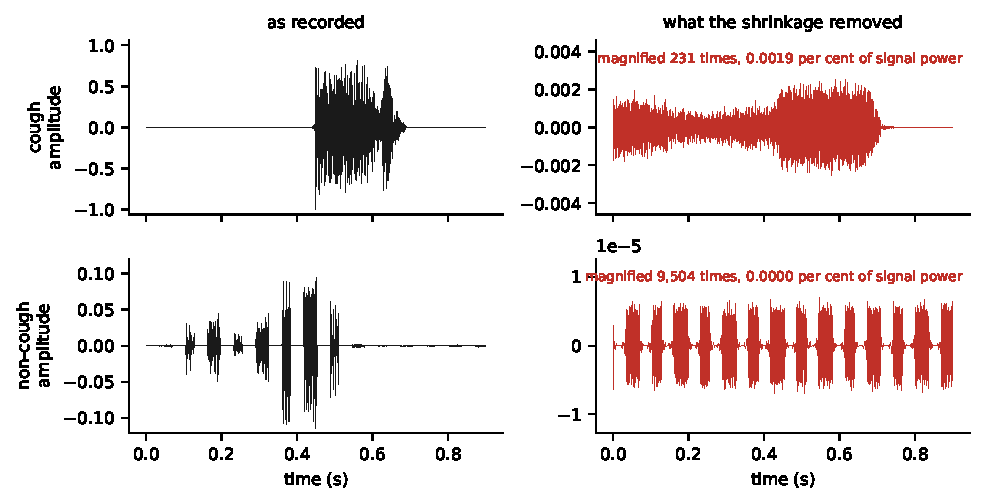
\includegraphics[width=\textwidth]{denoise.pdf}
\caption{What the universal threshold removes from one cough and one non-cough
recording.}\label{fig:denoise}
\end{figure*}

\subsection{Spectrogram formation and the frequency axis}\label{sec:design-spectro}

Each waveform is resampled to $16$~kHz and a short time Fourier transform is taken with a
$512$ point window and a hop of $256$ samples, giving $257$ frequency bins. Magnitudes
are converted to decibels. Two conditions differ only in what happens next, and this is
the second variable of the study.

In the linear condition the $257$ bins are used as they are. In the mel condition they are
mapped onto $128$ bands spaced on the mel scale of Stevens, Volkmann and
Newman~\cite{stevens1937}, which spaces bands according to perceived rather than physical
pitch and so allocates more resolution to low frequencies:
\begin{equation}
m(f) = 2595 \log_{10}\!\left(1 + \frac{f}{700}\right).
\label{eq:mel}
\end{equation}
The filterbank is triangular and follows the formulation used in hidden Markov model
toolkits. One property of it is worth stating because it bears on how much the mel
condition can differ from the linear one: at this configuration $128$ bands are requested
over $257$ bins, and one of the $128$ triangular filters contains no bin centre at all and
is therefore empty. The mel axis here is oversampled relative to the resolution the
transform provides, so the two conditions differ less in information content than the
change of axis suggests.

Both conditions produce a single channel image, which is resized to $224 \times 224$ and
replicated across three channels so that networks pretrained on photographs can accept
it. The conversion from decibels to pixel values is per recording, which means absolute
loudness is discarded and only the pattern within a recording survives.

\subsection{Networks}\label{sec:design-nets}

Four networks are used, chosen so that capacity and initialisation vary while the input
does not. Three are pretrained on ImageNet~\cite{russakovsky2015} and have their final
classification layer replaced by a two way layer: ResNet18~\cite{he2016}, which supplies
residual connections at modest depth, MobileNetV2~\cite{sandler2018}, which uses inverted
residuals and depthwise convolutions and is an order of magnitude smaller in multiply
accumulate operations, and DenseNet201~\cite{huang2017}, which is far deeper and
concatenates features across layers. The fourth is a compact network trained from random
initialisation, consisting of three blocks of convolution, batch normalisation,
rectification and max pooling, followed by a fully connected layer with dropout.

The fourth network exists to separate two things the work being extended could not. Its
baseline differed from its denoised condition in architecture, in pretraining, in the
frequency axis, and in the sample rate at once, so no single cause could be assigned to
the gap between them. Here the from scratch network sees exactly the images the
pretrained networks see, so the contribution of pretraining is isolated from the
contribution of the input.

All four are trained with Adam~\cite{kingma2015} in PyTorch~\cite{paszke2019}. The batch
size is the only hyperparameter that varies by network, and it varies for a hardware
reason rather than a modelling one: DenseNet201 activations at this input size do not fit
alongside the resident images in the available memory at a larger batch.

\section{Experimental setup}\label{sec:setup}

This section states what was run and how it is judged, in five parts:
Section~\ref{sec:setup-corpora} describes the three corpora and the label regime each
one represents, Section~\ref{sec:setup-split} the partitioning and why it is built around
participants rather than recordings, Section~\ref{sec:setup-train} the training protocol,
Section~\ref{sec:setup-metrics} the metrics and the statistical procedure, and
Section~\ref{sec:setup-repro} what one run consists of end to end together with the size
of the grid.

\subsection{Corpora and label provenance}\label{sec:setup-corpora}

A cough label can be obtained in at least three ways, and the three are treated here as
separate conditions rather than as interchangeable sources of ground truth. Table
\ref{tab:corpora} sets out the three corpora, what the positive and negative classes
consist of in each, and how the label was arrived at. The distinction is the organising
idea of the study, so it is worth stating plainly what each regime does and does not
establish.

\begin{table*}[tbp]
\caption{The three corpora, how the cough label was arrived at in each, and what the two classes consist of.}\label{tab:corpora}
\small
\begin{tabular}{@{}lp{0.11\textwidth}p{0.15\textwidth}p{0.17\textwidth}rrc@{}}
\toprule
Corpus & Label from & Positive class & Negative class & Recs. & Prior & Spk.\ ids \\
\midrule
Coswara & a prompt & the two cough tasks, heavy and shallow & breathing, sustained vowel
  and counting tasks & $13{,}314$ & $0.2228$ & yes \\
\addlinespace
FSD50K eval & a person & the \textsf{Cough} label & breathing, sneeze, gasp, sigh,
  laughter, speech & $476$ & $0.2227$ & no \\
\addlinespace
COUGHVID v3 & a detector & \texttt{cough\_detected} $\geq 0.9$ &
  \texttt{cough\_detected} $\leq 0.1$ & $8{,}398$ & $0.2239$ & no \\
\bottomrule
\end{tabular}
\end{table*}

\textbf{Prompt derived labels.} Coswara~\cite{coswara2020} records each participant
performing a sequence of prescribed vocal tasks. A recording is labelled cough because
the participant was asked to cough into the microphone, not because anyone listened to
it. The positive class is the two cough tasks, heavy and shallow, and the negative class
is the breathing, sustained vowel and counting tasks. Two properties make this the corpus
the main experiments run on. It carries a participant identifier, which makes a speaker
disjoint partition possible, and both classes come from the same participant, device and
recording session, so a difference between the classes cannot be explained by channel or
speaker.

\textbf{Human annotated labels.} FSD50K~\cite{fsd50k2022} consists of material annotated
by people against the AudioSet ontology~\cite{gemmeke2017}, and its evaluation split was
exhaustively verified by the corpus authors. Only that split is used, and it is never
trained on. Its value here is twofold: the label means a human judged a cough to be
present, and the ontology provides negatives that are deliberately confusable, since
breathing, sneezing, gasping, sighing and laughter are separate classes that can be
selected for rather than left to chance. A detector that only separates coughing from
silence is not worth reporting, and this is the set that tests whether more than that has
been achieved. Other collections of human annotated vocal sounds exist and carry cough
among their classes~\cite{vocalsound2022}; this split was preferred because its labels
were exhaustively verified by the corpus authors rather than sampled for verification, and
because the released audio of the alternative could not be retrieved from its distribution
point at the time of writing.

\textbf{Classifier derived labels.} COUGHVID~\cite{coughvid2021} ships a
\texttt{cough\_detected} score produced by the corpus authors' own detector, and provides
no human cough or non-cough judgement for the corpus as a whole. A model trained and
tested on labels thresholded from that score is measured on its agreement with that
detector, not on whether a cough is present. This is reported as a property of the
regime rather than worked around, because it is the regime a large part of the published
literature on this corpus operates in.

Two further facts about COUGHVID are recorded here because they constrain what can be
concluded from it. The recordings carry anonymous identifiers and no participant field,
so a speaker disjoint partition cannot be constructed and any contributor who submitted
more than once may appear on both sides of a split. And the selection used by the work
being extended cannot be reproduced from the corpus as published. That work reports
$15{,}619$ cough and $7{,}261$ non-cough recordings, $22{,}880$ retained of $34{,}434$.
The lower figure is reproducible: a threshold of $0.1271$ on \texttt{cough\_detected}
yields exactly $7{,}261$. The upper figure is not reproducible by any threshold on that
column, because six recordings carry the value $0.8961$ exactly, so the count at or above
a threshold near there steps from $15{,}617$ directly to $15{,}623$ and $15{,}619$ lies
strictly between the two. Something further was applied that the original does not
record. Rather than tune a near miss, this work uses round thresholds and states them:
a score of $0.9$ or above is taken as cough and $0.1$ or below as non-cough, with the
interval between them discarded, which retains $22{,}003$ of $34{,}434$ recordings.

Because the two corpora differ sharply in class prior, the COUGHVID arm is subsampled to
the prior of the Coswara arm, keeping every non-cough recording and sampling the cough
class down. Without this the two regimes would differ in task difficulty as well as in
label provenance, and the comparison would not isolate what it is meant to isolate.

\subsection{Partitioning}\label{sec:setup-split}

The Coswara partition is built over participants, not recordings. Participants are
assigned to the training, validation and test partitions in the proportions $70$, $15$ and
$15$ per cent, stratified by reported status and by the number of cough recordings
contributed, under a fixed seed. Every recording from a participant follows that
participant, and the builder asserts that the three participant sets are pairwise
disjoint before it writes the manifest, so the property is enforced rather than intended.
One manifest serves all four conditions, so the conditions are compared on identical
partitions.

This is not a refinement. A partition made over recordings allows one contributor to
appear in both training and test material, which makes part of the test set a memory
test. The scale of the effect has been measured before: a mel spectrogram convolutional
network reported $98.18$ per cent accuracy under a random split and $95.18$ per cent when
test coughs came from recordings unseen in training~\cite{zhou2021}, a gap of roughly
three points which that work reported without discussing. Evidence from respiratory audio
more broadly points the same way. Audio classifiers that appeared accurate on
crowdsourced material fell from $0.846$ to $0.619$ area under the curve once confounders
including self-reported symptoms were matched~\cite{coppock2024}, and a careful evaluation
of the same kind of data reached $0.71$ where a less careful one reached
$0.90$~\cite{han2022}. A recent cross-dataset study of cough models found that their
learned representations cluster by recording device and corpus rather than by the
condition being detected~\cite{zhang2026}, which is the mechanism these gaps would be
expected to arise from. Two of its authors are also authors of
COUGHVID~\cite{coughvid2021}.

For COUGHVID the partition is over recordings, for the reason given in
Section~\ref{sec:setup-corpora}, and that limitation attaches to every number reported
for that arm. FSD50K is used only for evaluation, so it is not partitioned at all.

\subsection{Training protocol}\label{sec:setup-train}

One protocol is applied identically to every run. Each network is trained with
Adam~\cite{kingma2015} at a learning rate of $10^{-4}$ for at most eight epochs, with
gradients clipped to unit norm. Training stops early when validation balanced accuracy
has failed to improve for three consecutive epochs. The weights retained are those from
the epoch with the best validation balanced accuracy, selected without any reference to
the test partition, and the test partition is read exactly once per run, after selection.
Computation is in single precision. Table~\ref{tab:training} gives the full settings, in which the batch size is the only entry that varies with architecture, for the reason given below.

Three of these choices are consequences of observed failures rather than preferences.
Gradient clipping is present because an unclipped run at the learning rate inherited from
the work being extended diverges to a non-finite loss on this hardware. Single precision
is used because mixed precision produced a non-finite loss from the first optimiser step:
at the gradient scaler's initial scale the gradients of the first convolution overflow
the half precision range, and clipping then divides by an infinite norm and writes
non-finite values into the gradients after the scaler's own overflow check has already
run. The network never leaves the majority class, and the resulting accuracy equals the
majority class frequency exactly. The trainer counts and reports any optimiser step it
has to abandon for a non-finite gradient norm, so this mode of failure cannot pass for a
successful run.

A third choice follows from a measurement rather than a preference, and it concerns the
batch size, which is set per architecture. The driver on the development hardware does
not refuse an allocation that exceeds the four gigabytes of device memory. It satisfies
the excess from host memory instead, and the traffic then crosses the system bus on every
access. Nothing fails, no warning is issued, and the only symptom is throughput.
MobileNetV2 at a batch of $64$ reserves $5450$ MiB and trains at $23$ images per second,
while the same network at $16$ reserves $2228$ MiB and trains at $148$, a factor of
$6.4$ for a quantity that appears in no diagnostic. DenseNet201 shows the same effect
more sharply, $1.6$ images per second at a batch of $32$ against $29.8$ at $8$. Inverted
residuals and dense concatenation are what make these two the binding cases, since both
keep high resolution feature maps alive across many layers, so the activation memory of
each is far larger than its operation count would suggest. The competing explanation,
that the depthwise separable convolutions were reaching a slow kernel, was tested by
repeating every measurement in the channels last memory layout and is rejected: that
layout leaves the peak essentially unchanged and runs an order of magnitude slower again,
and a remedy that raises throughput without lowering the peak was not addressing a memory
problem. The batch for each architecture is therefore set to leave roughly a gigabyte of
the card unused rather than to the largest value that happens to fit, because the
quantity being protected is a peak and the rest of the machine is in use.
Table~\ref{tab:throughput} gives the measurements the choice rests on. The card holds $4096$~MiB; a peak above that figure is not an error on this platform, because the excess is served from host memory, and the channels last rows show that the memory layout does not address the cause.

\begin{table}[htbp]
\caption{Training protocol, applied identically to every run.}\label{tab:training}
\small
\begin{tabular}{@{}lp{0.55\columnwidth}@{}}
\toprule
Setting & Value \\
\midrule
Optimiser & Adam, learning rate $10^{-4}$ \\
Gradient clipping & unit norm \\
Epochs & at most $8$ \\
Early stopping & no gain in validation balanced accuracy for $3$ epochs \\
Weights retained & those of the best validation balanced accuracy epoch \\
Test reads per run & one, after selection \\
Precision & single \\
Input & $224 \times 224$, normalised by ImageNet channel statistics \\
Batch size & $64$ ResNet18, $16$ MobileNetV2, $128$ compact, $8$ DenseNet201 \\
Seeds & five, and three for DenseNet201 \\
\bottomrule
\end{tabular}
\end{table}

\begin{table}[htbp]
\caption{Training throughput and peak reserved device memory, per architecture.}\label{tab:throughput}
\small
\begin{tabular}{@{}llrrr@{}}
\toprule
Architecture & Layout & Batch & Images/s & Peak MiB \\
\midrule
ResNet18 & contiguous & $64$ & $208.1$ & $2898$ \\
\addlinespace
MobileNetV2 & contiguous & $64$ & $23.2$ & $5450$ \\
MobileNetV2 & contiguous & $32$ & $148.4$ & $3222$ \\
MobileNetV2 & contiguous & $16$ & $147.6$ & $2228$ \\
MobileNetV2 & channels last & $32$ & $13.2$ & $3254$ \\
MobileNetV2 & channels last & $16$ & $14.8$ & $2238$ \\
\addlinespace
Compact & contiguous & $128$ & $967.1$ & $3098$ \\
Compact & contiguous & $64$ & $912.6$ & $1608$ \\
\addlinespace
DenseNet201 & contiguous & $32$ & $1.6$ & $7372$ \\
DenseNet201 & contiguous & $12$ & $33.6$ & $3070$ \\
DenseNet201 & contiguous & $8$ & $29.8$ & $2284$ \\
\bottomrule
\end{tabular}
\end{table}

\subsection{Metrics and statistical procedure}\label{sec:setup-metrics}

Accuracy alone is not adequate on these class priors, so balanced accuracy, specificity
and the Matthews correlation coefficient~\cite{matthews1975} are reported alongside it.
The correlation coefficient is included because it responds to all four cells of the
confusion matrix in proportion to both class sizes, which accuracy and the harmonic mean
of precision and recall do not~\cite{chicco2020}. Interval estimates use the Wilson score
interval~\cite{wilson1927} rather than the Wald interval, whose coverage is erratic at
proportions near one~\cite{brown2001}, which is the region every condition here occupies.

Differences between conditions are tested on paired decisions, not on accuracies. For a
pair of conditions evaluated on the same test recordings under the same seed, the
quantities of interest are the counts of recordings that one condition classifies
correctly and the other does not, and these are assessed with McNemar's
test~\cite{mcnemar1947}, exactly while the discordant total is small enough to enumerate
and by the continuity corrected approximation otherwise. Of five tests compared for this
purpose, McNemar's was the only one with an acceptable Type I error rate for a learner
that is trained once~\cite{dietterich1998}. Because a family of such comparisons is made,
the p values are adjusted by the step down procedure of Holm~\cite{holm1979}.

One further quantity is reported beside every effect, and it governs how the effects
should be read. Each condition is run under five seeds, three in the case of DenseNet201,
and the spread of accuracy across those seeds is reported. An effect smaller than roughly
twice that spread cannot be claimed from single runs, however large the test set is. The
spread quoted for DenseNet201 rests on three runs and is accordingly a coarser estimate
than the others, which is a further reason not to read a small difference involving it as
an effect. This is stated because
differences well under one accuracy point are routinely reported in this area without any
estimate of run to run variation, and the present work is in a position to say what that
variation is.

\subsection{Reproducibility}\label{sec:setup-repro}

A single run consists of the following, end to end. The images for one condition are
loaded for all three partitions and held in device memory as unsigned bytes, converted to
normalised single precision per batch. One architecture is trained from one seed under
the protocol of Section~\ref{sec:setup-train}. The epoch with the best validation
balanced accuracy is restored, the test partition is evaluated once, and one row per test
recording is written out carrying the file identifier, the true label, the predicted
label and both class scores. Those rows, not any summary of them, are what the analysis
reads, which is what makes the paired tests of Section~\ref{sec:setup-metrics} possible
at all.

The grid over the prompt derived corpus is $66$ runs. ResNet18, MobileNetV2 and the
compact network are each run on all four conditions under five seeds, which is $60$ runs,
and DenseNet201 is run on the two mel conditions under three seeds, which is a further
six; its batch size constraint makes it several times more expensive per run than the
others. The four conditions are the two frequency axes crossed with denoising applied or
withheld.

Three secondary experiments are reported, each settling one question.
\begin{enumerate}
\item Whether the accuracy obtained on prompted recordings survives a change of corpus,
      annotator and negative class. Settled by evaluating the retained networks on the
      human annotated evaluation split without retraining, in
      Section~\ref{sec:res-external}.
\item Whether the label regime changes the answer about denoising. Settled by repeating
      the ResNet18 block on the classifier derived corpus at a matched class prior, in
      Section~\ref{sec:res-regime}.
\item Whether the expert annotated subset of the classifier derived corpus can be used to
      estimate its label error rate. Settled in the negative, in
      Section~\ref{sec:res-regime}, because that subset is not a random sample of the
      corpus.
\end{enumerate}

Every count in this section and in Section~\ref{sec:results} is derived from the saved
decision files by script rather than by arithmetic on the page, and the scripts that do
so are released with the code.

\section{Results}\label{sec:results}

The results are reported in the order the questions were posed.
Section~\ref{sec:res-grid} gives the grid over the prompt derived corpus, which establishes
what the pipeline achieves when it is trained and tested in the usual way.
Section~\ref{sec:res-denoise} tests the preprocessing step the work being extended relies
on. Section~\ref{sec:res-external} applies the retained weights to human annotated audio
without retraining, which is the test the earlier evaluation did not make.
Section~\ref{sec:res-regime} reports what can and cannot be established from the
classifier derived corpus. Section~\ref{sec:res-limits} states what the results do not
support. Every figure quoted below is computed from the saved per recording decisions by
the scripts released with the code, and the tables are generated from those same files.

\subsection{Detection within the prompt derived corpus}\label{sec:res-grid}

Table~\ref{tab:grid} gives the grid. ResNet18 reaches $99.09 \pm 0.13$ per cent accuracy
on the linear condition, with sensitivity $97.72 \pm 0.62$ and specificity
$99.48 \pm 0.26$, for a balanced accuracy of $98.60 \pm 0.22$ and a correlation
coefficient of $0.974 \pm 0.004$. These are the numbers the literature reports for this
task, obtained here under a partition in which no participant appears on both sides of a
split, so the simplest explanation for a high score is excluded: the networks are not
recognising speakers they were trained on.

\begin{table*}[tbp]
\caption{Detection on the prompt derived corpus, over held out speakers.}\label{tab:grid}
\small
\begin{tabular}{@{}llrcccc@{}}
\toprule
Architecture & Input & Seeds & Accuracy & Sensitivity & Specificity & MCC \\
\midrule
ResNet18 & linear & 5 & $99.09 \pm 0.13$ & $97.72 \pm 0.62$ & $99.48 \pm 0.26$ & $0.974 \pm 0.004$ \\
 & wav+linear & 5 & $98.80 \pm 0.24$ & $97.14 \pm 0.53$ & $99.27 \pm 0.30$ & $0.965 \pm 0.007$ \\
 & mel & 5 & $98.71 \pm 0.20$ & $97.19 \pm 0.81$ & $99.14 \pm 0.10$ & $0.963 \pm 0.006$ \\
 & wav+mel & 5 & $98.65 \pm 0.49$ & $97.37 \pm 0.53$ & $99.02 \pm 0.74$ & $0.961 \pm 0.014$ \\
\addlinespace
MobileNetV2 & linear & 5 & $99.10 \pm 0.12$ & $97.68 \pm 0.97$ & $99.50 \pm 0.28$ & $0.974 \pm 0.003$ \\
 & wav+linear & 5 & $98.89 \pm 0.16$ & $97.01 \pm 1.08$ & $99.43 \pm 0.42$ & $0.968 \pm 0.004$ \\
 & mel & 5 & $98.86 \pm 0.33$ & $98.35 \pm 0.34$ & $99.00 \pm 0.49$ & $0.967 \pm 0.009$ \\
 & wav+mel & 5 & $98.91 \pm 0.23$ & $97.50 \pm 0.91$ & $99.31 \pm 0.30$ & $0.968 \pm 0.007$ \\
\addlinespace
DenseNet201 & mel & 3 & $99.07 \pm 0.12$ & $97.92 \pm 0.68$ & $99.40 \pm 0.13$ & $0.973 \pm 0.004$ \\
 & wav+mel & 3 & $98.73 \pm 0.50$ & $97.54 \pm 0.59$ & $99.06 \pm 0.78$ & $0.964 \pm 0.014$ \\
\addlinespace
Compact & linear & 5 & $96.43 \pm 0.38$ & $93.35 \pm 1.60$ & $97.31 \pm 0.74$ & $0.898 \pm 0.010$ \\
 & wav+linear & 5 & $95.62 \pm 0.30$ & $92.37 \pm 1.71$ & $96.55 \pm 0.47$ & $0.876 \pm 0.009$ \\
 & mel & 5 & $96.46 \pm 0.34$ & $92.46 \pm 2.24$ & $97.60 \pm 0.83$ & $0.898 \pm 0.009$ \\
 & wav+mel & 5 & $92.57 \pm 8.29$ & $73.93 \pm 41.40$ & $97.89 \pm 1.55$ & $0.715 \pm 0.400$ \\
\bottomrule
\end{tabular}
\end{table*}

The compact network reaches $96.43 \pm 0.38$ per cent on the same condition, and the gap
between it and ResNet18 is larger in sensitivity, $93.35 \pm 1.60$ against
$97.72 \pm 0.62$, than in specificity, where the two are within a point and a half of each
other. Capacity is therefore being spent on recovering coughs rather than on rejecting the
negatives, which is consistent with a negative class that is not difficult.

One result in the table is a failure rather than a measurement, and it is reported because
it bears on the stability of the smaller network. The compact network on the wavelet
shrunk mel condition averages $73.93 \pm 41.40$ per cent sensitivity. A standard deviation
of that size on a quantity bounded by one hundred is not a spread about a mean; it records
that the seeds did not all produce the same kind of model. One seed converged to the
majority class and stayed there, which on this prior produces an accuracy equal to the
non-cough frequency and a sensitivity of zero. The trainer reports any optimiser step
abandoned for a non-finite gradient, and none were abandoned in that run, so this is an
optimisation outcome rather than the arithmetic failure described in
Section~\ref{sec:setup-train}. The relevant observation is that it happened under the
condition combining the mel axis with shrinkage and under no other, and only to the
network with the least capacity.

DenseNet201 was run on the two mel conditions at three seeds, because its memory
requirement makes it several times more expensive per run than the others, and what it
shows is worth that cost. On the mel axis it reaches $98.66 \pm 0.31$ per cent balanced
accuracy, against MobileNetV2's $98.68 \pm 0.17$ and ResNet18's $98.17 \pm 0.41$. The
deepest network in the comparison is therefore indistinguishable from the smallest
pretrained one, and its margin over the middle one is half a point, which is inside the
bound Section~\ref{sec:setup-metrics} sets for an effect that may be claimed at all. The
separation that does appear is the three to four points between each of the three
pretrained networks and the one trained from random initialisation on the same axis. On
this task, at this label quality, it is pretrained initialisation and not capacity that
distinguishes one architecture from another.

\subsection{Whether wavelet shrinkage helps}\label{sec:res-denoise}

Table~\ref{tab:paired} tests the shrinkage on paired decisions. The result is that it does
not help, and that where the effect reaches significance it is negative. \figref{fig:effect} sets each effect against the spread across seeds it would have to clear to be claimable from single runs, and most of them fall on the wrong side of that line.

\begin{table*}[tbp]
\caption{Wavelet shrinkage tested on paired decisions over the prompt derived corpus.}\label{tab:paired}
\small
\begin{tabular}{@{}llrrrllc@{}}
\toprule
Architecture & Comparison & Seeds & $b$ & $c$ & $p$ & $p$ adj.\ & Accuracy change \\
\midrule
ResNet18 & linear $\rightarrow$ wav+linear & 5 & 66 & 37 & $0.0055$ & $0.0277$ & $-0.29 \pm 0.19$ \\
ResNet18 & mel $\rightarrow$ wav+mel & 5 & 71 & 65 & $0.668$ & $1.000$ & $-0.06 \pm 0.39$ \\
MobileNetV2 & linear $\rightarrow$ wav+linear & 5 & 71 & 50 & $0.0686$ & $0.206$ & $-0.21 \pm 0.24$ \\
MobileNetV2 & mel $\rightarrow$ wav+mel & 5 & 53 & 58 & $0.704$ & $1.000$ & $+0.05 \pm 0.40$ \\
DenseNet201 & mel $\rightarrow$ wav+mel & 3 & 50 & 29 & $0.0238$ & $0.0953$ & $-0.35 \pm 0.52$ \\
Compact & linear $\rightarrow$ wav+linear & 5 & 196 & 115 & $<10^{-4}$ & $<10^{-4}$ & $-0.80 \pm 0.65$ \\
Compact & mel $\rightarrow$ wav+mel & 5 & 525 & 133 & $<10^{-4}$ & $<10^{-4}$ & $-3.89 \pm 8.25$ \\
\bottomrule
\end{tabular}
\end{table*}

\begin{figure}[tbp]
\centering
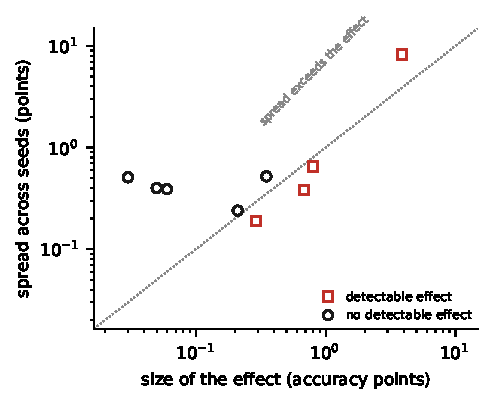
\includegraphics[width=0.98\columnwidth]{effect.pdf}
\caption{Each shrinkage effect against the seed spread it would have to clear.}\label{fig:effect}
\end{figure}

For ResNet18 on the linear axis, $66$ recordings are classified correctly without
shrinkage and incorrectly with it, against $37$ in the reverse direction. McNemar's test
on those discordant pairs gives $p = 0.0055$, which survives the step down correction over
the family in Table~\ref{tab:paired}, and the accuracy change across seeds is
$-0.29 \pm 0.19$ points. The effect is therefore real, small, and in the direction
opposite to the one claimed for the method. On the mel axis the same comparison is
indistinguishable from no effect, $71$ against $65$ discordant recordings and
$p = 0.668$ before any correction. For the compact network on the mel axis the test
rejects decisively, but the accuracy change is $-3.89 \pm 8.25$ points, and a spread four
times the size of the effect is the degenerate seed discussed above rather than a property
of shrinkage. The same network on the linear axis carries the same conclusion without that
complication: $196$ recordings against $115$, a decisive rejection, and a change of
$-0.80 \pm 0.65$ points with no degenerate seed behind it.

DenseNet201 contributes the one comparison that shows what the correction is for. Its
single test gives $p = 0.0238$, which any convention that ignores the family a test
belongs to would report as an effect, and $0.0953$ after the step down, which would not.
Had that architecture been run on its own, the same decisions would have been published as
a significant result about shrinkage on the mel axis, and over the family they do not
support one.

Section~\ref{sec:design-denoise} supplies the mechanism, and it is worth restating here
because it determines how far these results generalise. The universal threshold is set
from an estimate of the noise level in the finest detail coefficients. On recordings
already as clean as these it falls far below the signal, and the measured consequence is
that a median of $0.67$ per cent of signal power is removed, with quartiles at $0.08$ and
$2.28$ per cent. The two input conditions are therefore very nearly the same images, and
the null result is what should be expected rather than a surprise. This is a statement
about applying this family of shrinkage rules to corpora of this quality; it is not
evidence that denoising cannot help audio that is genuinely noisy.

\subsection{Transfer to human annotated audio}\label{sec:res-external}

The weights retained from the grid were applied, without retraining and without adaptation
of any kind, to the exhaustively verified evaluation split of the human annotated corpus
at the same class prior. Table~\ref{tab:external} gives the result, its rows corresponding one to one with
those of Table~\ref{tab:grid}, and \figref{fig:transfer} plots it against the in corpus
figure for the same weights. In that figure the dotted line marks equal performance and
the error bars are one standard deviation across seeds on each axis; the input
conditions run for each architecture are plotted without being labelled separately,
because they fall on top of one another, the choice of frequency axis and the presence
or absence of shrinkage moving the result by far less than the change of corpus does.
The fall itself is asymmetric: specificity is substantially retained while sensitivity
is not, so the detectors go on rejecting non-coughs and stop recovering coughs.

\begin{table*}[tbp]
\caption{The saved weights on human annotated audio at a matched class prior, without retraining. Rows match Table~\ref{tab:grid}.}\label{tab:external}
\small
\begin{tabular}{@{}llrcccc@{}}
\toprule
Architecture & Input & Seeds & Accuracy & Sensitivity & Specificity & MCC \\
\midrule
ResNet18 & linear & 5 & $78.03 \pm 1.62$ & $56.04 \pm 4.04$ & $84.32 \pm 3.24$ & $0.391 \pm 0.012$ \\
 & wav+linear & 5 & $79.33 \pm 1.19$ & $53.21 \pm 1.27$ & $86.81 \pm 1.65$ & $0.402 \pm 0.022$ \\
 & mel & 5 & $78.70 \pm 2.31$ & $57.55 \pm 3.89$ & $84.76 \pm 3.88$ & $0.411 \pm 0.031$ \\
 & wav+mel & 5 & $77.56 \pm 3.18$ & $59.62 \pm 2.78$ & $82.70 \pm 4.34$ & $0.401 \pm 0.056$ \\
\addlinespace
MobileNetV2 & linear & 5 & $78.15 \pm 2.28$ & $60.57 \pm 5.48$ & $83.19 \pm 4.26$ & $0.415 \pm 0.024$ \\
 & wav+linear & 5 & $76.26 \pm 2.85$ & $56.04 \pm 3.92$ & $82.05 \pm 4.46$ & $0.362 \pm 0.039$ \\
 & mel & 5 & $74.92 \pm 3.98$ & $66.04 \pm 4.11$ & $77.46 \pm 5.97$ & $0.392 \pm 0.054$ \\
 & wav+mel & 5 & $77.65 \pm 3.00$ & $57.92 \pm 4.30$ & $83.30 \pm 4.89$ & $0.396 \pm 0.038$ \\
\addlinespace
DenseNet201 & mel & 3 & $81.09 \pm 1.31$ & $54.40 \pm 2.37$ & $88.74 \pm 2.03$ & $0.443 \pm 0.025$ \\
 & wav+mel & 3 & $74.72 \pm 7.96$ & $59.43 \pm 7.37$ & $79.10 \pm 11.65$ & $0.364 \pm 0.096$ \\
\addlinespace
Compact & linear & 5 & $68.11 \pm 1.55$ & $45.66 \pm 4.88$ & $74.54 \pm 3.26$ & $0.184 \pm 0.015$ \\
 & wav+linear & 5 & $69.92 \pm 5.44$ & $43.40 \pm 6.26$ & $77.51 \pm 8.62$ & $0.202 \pm 0.052$ \\
 & mel & 5 & $73.36 \pm 5.67$ & $38.49 \pm 9.70$ & $83.35 \pm 10.00$ & $0.235 \pm 0.049$ \\
 & wav+mel & 5 & $70.34 \pm 8.57$ & $36.79 \pm 21.85$ & $79.95 \pm 16.25$ & $0.161 \pm 0.106$ \\
\bottomrule
\end{tabular}
\end{table*}

ResNet18 on the linear condition falls from $98.60$ per cent balanced accuracy to
$70.18 \pm 0.44$. The fall is not uniform across the two classes, and the asymmetry is the
substantive finding. Specificity declines from $99.48 \pm 0.26$ to $84.32 \pm 3.24$, which
is a real loss but leaves the detector still rejecting most non-coughs. Sensitivity falls
from $97.72 \pm 0.62$ to $56.04 \pm 4.04$. A detector that recovered better than ninety
seven coughs in a hundred within the corpus it was fitted to recovers barely more than
half of them once the recordings, the microphones, the annotators and the definition of
the negative class all change together.

\begin{figure*}[tbp]
\centering
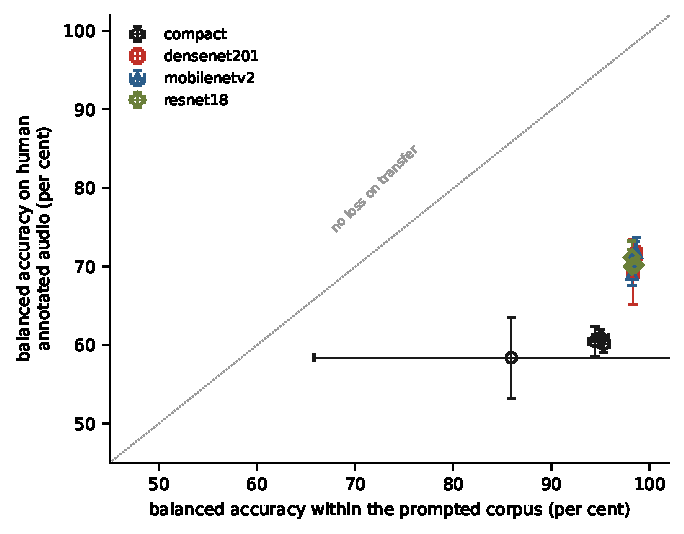
\includegraphics[width=0.74\textwidth]{transfer.pdf}
\caption{In corpus against out of corpus balanced accuracy for the same saved
weights.}\label{fig:transfer}
\end{figure*}

A fall of this size has two possible causes that call for quite different responses, and
they can be told apart. The networks may have stopped ranking coughs above non-coughs, in
which case the representation does not transfer and nothing applied after the fact will
recover it. Or they may still rank them correctly while the decision threshold inherited
from training now sits in the wrong place, in which case the loss is a calibration problem
and a practitioner holding a little labelled data from the target domain can fix it
cheaply. The area under the receiver operating characteristic distinguishes the two,
because it depends on the ordering of the scores alone and not on where the threshold
falls. Table~\ref{tab:threshold} reports it.

\begin{table*}[tbp]
\caption{Discrimination against calibration on the external set.}\label{tab:threshold}
\small
\begin{tabular}{@{}llcccc@{}}
\toprule
& & \multicolumn{2}{c}{Area under the curve} & \multicolumn{2}{c}{External balanced accuracy} \\
\cmidrule(lr){3-4}\cmidrule(lr){5-6}
Architecture & Input & In corpus & External & At $0.5$ & Best possible \\
\midrule
ResNet18 & linear & $0.998 \pm 0.002$ & $0.749 \pm 0.018$ & $70.18 \pm 0.44$ & $71.90 \pm 0.91$ \\
 & wav+linear & $0.998 \pm 0.001$ & $0.730 \pm 0.007$ & $70.01 \pm 0.81$ & $71.13 \pm 0.52$ \\
 & mel & $0.999 \pm 0.000$ & $0.768 \pm 0.016$ & $71.15 \pm 1.01$ & $72.34 \pm 1.68$ \\
 & wav+mel & $0.998 \pm 0.001$ & $0.754 \pm 0.024$ & $71.16 \pm 2.08$ & $72.31 \pm 1.35$ \\
\addlinespace
MobileNetV2 & linear & $0.998 \pm 0.000$ & $0.768 \pm 0.007$ & $71.88 \pm 1.25$ & $73.30 \pm 0.73$ \\
 & wav+linear & $0.998 \pm 0.001$ & $0.739 \pm 0.014$ & $69.05 \pm 1.45$ & $70.61 \pm 1.95$ \\
 & mel & $0.998 \pm 0.000$ & $0.766 \pm 0.025$ & $71.75 \pm 1.93$ & $72.90 \pm 1.62$ \\
 & wav+mel & $0.998 \pm 0.001$ & $0.748 \pm 0.023$ & $70.61 \pm 1.17$ & $71.64 \pm 1.65$ \\
\addlinespace
DenseNet201 & mel & $0.998 \pm 0.001$ & $0.767 \pm 0.022$ & $71.57 \pm 0.96$ & $72.96 \pm 0.93$ \\
 & wav+mel & $0.998 \pm 0.002$ & $0.736 \pm 0.021$ & $69.27 \pm 4.09$ & $70.99 \pm 3.07$ \\
\addlinespace
Compact & linear & $0.992 \pm 0.001$ & $0.648 \pm 0.012$ & $60.10 \pm 1.06$ & $62.23 \pm 1.59$ \\
 & wav+linear & $0.988 \pm 0.002$ & $0.650 \pm 0.019$ & $60.45 \pm 1.87$ & $62.81 \pm 1.52$ \\
 & mel & $0.993 \pm 0.000$ & $0.687 \pm 0.017$ & $60.92 \pm 1.01$ & $64.36 \pm 1.58$ \\
 & wav+mel & $0.985 \pm 0.012$ & $0.651 \pm 0.028$ & $58.37 \pm 5.18$ & $62.10 \pm 2.02$ \\
\bottomrule
\end{tabular}
\end{table*}

The answer is the unwelcome one. For ResNet18 on the linear condition the area under the
curve falls from $0.998$ within the corpus to $0.749$ outside it. The ordering itself has
degraded, and the threshold is very nearly where it ought to be: balanced accuracy at the
inherited threshold is $70.18$ per cent, while the best value attainable at any threshold
on this set is $71.90$. Recalibration could therefore recover about $1.7$ points, and even
that figure is optimistic, because the threshold achieving it was chosen on the same
recordings it is scored on and no procedure could have selected it in advance. The same
pattern holds for every architecture and condition in the table. The obvious and cheapest
remedy for a domain shift, collecting a little target data and moving the operating point,
would recover almost none of what was lost here.

Two further observations follow from the external table. The first is that the only
separation between architectures that was worth anything inside the corpus is also the
only one that survives leaving it, and it does not lie between the pretrained networks.
ResNet18, MobileNetV2 and DenseNet201 reach $71.15 \pm 1.01$, $71.75 \pm 1.93$ and
$71.57 \pm 0.96$ per cent balanced accuracy on the mel axis outside the corpus, which
places all three inside one another's spread, as they were inside it. The compact network,
roughly three points behind ResNet18 in corpus, is roughly ten points behind it out of
corpus, at $60.10 \pm 1.06$ on the linear condition. Whatever pretraining supplied that
the smaller network had to find in the data alone, part of it transfers, and capacity
beyond that supplies nothing in either regime. The second is that the input conditions remain
indistinguishable from one another under the change of corpus. Shrinkage gains
$1.30 \pm 1.36$ accuracy points on the linear axis externally, which is a change smaller
than its own spread across seeds, so the external set does not rescue the preprocessing
step either.

The degenerate seed reappears here and is worth following, because it shows what a single
run can conceal. The compact network on the wavelet shrunk mel condition records, for one
seed, an accuracy of $77.73$ per cent against a balanced accuracy of exactly $50.00$. The
first number is simply the proportion of non-coughs in the external set. The model
assigned every one of the $476$ recordings to the majority class, and an evaluation
reporting accuracy alone would have recorded it as the second best run of that condition.

Because the external negatives are annotated against the ontology, it is possible to ask
not merely how many false positives there are but what produces them.
Table~\ref{tab:confusion} gives the rate at which clips carrying each annotated class are
assigned to the cough class, pooled over every ResNet18 run, and \figref{fig:falsepos} orders the classes by that rate. A clip may carry several labels, so the rows overlap and their counts do not sum to the size of the negative class.

\begin{table}[htbp]
\caption{What the detectors call a cough, by annotated class, pooled over every ResNet18 run on the external set.}\label{tab:confusion}
\small
\begin{tabular}{@{}lrrc@{}}
\toprule
Annotated class & Decisions & Called cough & Per cent \\
\midrule
Sneeze & 360 & 244 & $67.8$ \\
Burping & 440 & 149 & $33.9$ \\
Whispering & 520 & 139 & $26.7$ \\
Gasp & 200 & 41 & $20.5$ \\
Sigh & 280 & 56 & $20.0$ \\
Breathing & 800 & 132 & $16.5$ \\
Yell & 280 & 40 & $14.3$ \\
Male speech & 2320 & 316 & $13.6$ \\
Speech & 4180 & 492 & $11.8$ \\
Laughter & 1400 & 161 & $11.5$ \\
Female speech & 1460 & 143 & $9.8$ \\
Child speech & 440 & 34 & $7.7$ \\
Chewing & 360 & 22 & $6.1$ \\
\addlinespace
Cough, as recall & 2120 & 1200 & $56.6$ \\
\bottomrule
\end{tabular}
\end{table}

\begin{figure}[tbp]
\centering
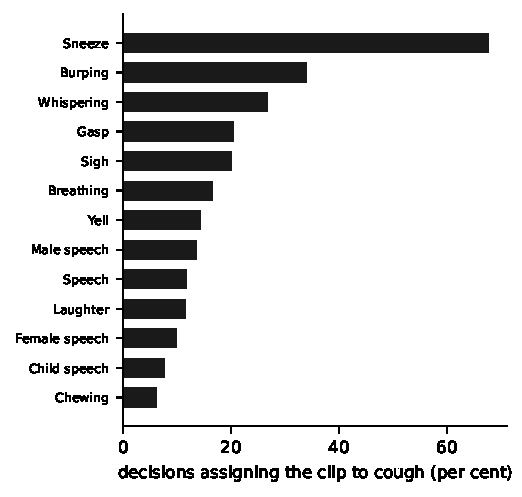
\includegraphics[width=0.98\columnwidth]{falsepos.pdf}
\caption{The rate at which each annotated class is assigned to the cough class.}\label{fig:falsepos}
\end{figure}

The errors are not spread evenly over the negative class, and the concentration is
severe. Clips labelled \textsf{Sneeze} are called coughs in $67.8$ per cent of decisions.
That is a higher rate than the detectors achieve on clips that really are coughs, where
recall over the same runs is $56.6$ per cent. On this evidence a sneeze is more likely to
be reported as a cough than a cough is. Burping follows at $33.9$ per cent, whispering at
$26.7$, gasping at $20.5$ and sighing at $20.0$, while breathing sits at $16.5$ and the
speech classes fall between $7.7$ and $13.6$.

The ordering is interpretable, and it is the one the construction of the prompted corpus
predicts. The sounds most readily confused with coughing are the other forced
expirations. A sneeze, a burp, a gasp and a sigh are each a sudden release of air through
the vocal tract, distinguished from a cough by details a detector has no reason to encode
if it was never required to. The negative class of the prompted corpus is breathing,
sustained vowels and counting, and not one of those is a forced expiration. A model
trained against it is never asked to separate coughing from sneezing, and the external
evaluation finds that it cannot. This is the mechanism behind the loss of discrimination
reported above, and it indicates what a corpus intended to support cough detection would
need to contain: not more recordings, but negatives that are hard in the particular way
that matters.

\subsection{What the classifier derived corpus can establish}\label{sec:res-regime}

The third regime is reported separately because the quantity it measures is different in
kind. A model trained and tested on labels thresholded from a detector score is measured on
its agreement with that detector. A high figure there is evidence that two classifiers
agree, which is not evidence that a cough is present, and no amount of care in the
partitioning changes what is being measured.

At the matched prior this corpus supplies $8398$ recordings, of which $1880$ carry a cough
label, and its test partition holds $1259$ of them. Within that regime a ResNet18 reaches
$98.41 \pm 0.24$ per cent balanced accuracy on linear spectrograms, against $98.60 \pm
0.22$ on the prompt derived corpus under the same architecture and the same input
condition. Table~\ref{tab:regime} gives the four conditions. The resemblance between those
two figures is the most instructive thing about them: a reader given only the headline
number could not tell which of the two experiments produced it, although one measures
recovery of a prompted behaviour from held out speakers and the other measures agreement
with a detector. Nothing in the quantity itself marks the difference, which is why the
regime is named in the caption rather than left to be inferred from the corpus name.

\begin{table*}[tbp]
\caption{Detection on the classifier derived corpus at a matched class prior.}\label{tab:regime}
\small
\begin{tabular}{@{}llrcccc@{}}
\toprule
Architecture & Input & Seeds & Accuracy & Sensitivity & Specificity & MCC \\
\midrule
ResNet18 & linear & 5 & $98.94 \pm 0.14$ & $97.45 \pm 0.68$ & $99.37 \pm 0.29$ & $0.969 \pm 0.004$ \\
 & wav+linear & 5 & $98.25 \pm 0.51$ & $97.87 \pm 1.00$ & $98.36 \pm 0.85$ & $0.951 \pm 0.013$ \\
 & mel & 5 & $98.57 \pm 0.32$ & $98.09 \pm 1.05$ & $98.71 \pm 0.52$ & $0.960 \pm 0.009$ \\
 & wav+mel & 5 & $98.60 \pm 0.25$ & $97.38 \pm 0.48$ & $98.96 \pm 0.36$ & $0.960 \pm 0.007$ \\
\bottomrule
\end{tabular}
\end{table*}

The paired test behaves on this corpus much as it does on the other. Shrinkage applied
before a linear spectrogram costs $0.68 \pm 0.38$ accuracy points, with $79$ recordings
lost against $36$ gained and an adjusted $p$ of $0.0002$; applied before a mel spectrogram
it changes nothing measurable, $51$ against $53$ and $p = 0.922$. The direction agrees
with the prompt derived corpus in both pairs and the magnitude is larger in the first,
which is consistent with shrinkage removing detail that the linear axis still resolves and
the mel axis has already averaged together. What a loss of agreement means here needs
stating, though. These labels were assigned to the recordings as distributed rather than to
shrunk versions of them, so a processing step that moves a model away from those labels has
not thereby been shown to move it away from the coughs.

This corpus also cannot support the partitioning the other two receive. It distributes no
participant identifier, so recordings contributed by one person cannot be kept to one side
of a split, and the figures in Table~\ref{tab:regime} are accordingly not protected against
a contributor appearing in both training and test. That is a second reason, independent of
the labels, to read them as a property of the regime rather than as a detection result.

Two properties of the corpus bound what can be done with it, and both are settled from the
published metadata without reference to any model. The first concerns reproducing the
selection used by the work being extended, which reports $15{,}619$ cough and $7{,}261$
non-cough recordings. The lower count is reachable: a threshold of $0.1271$ on the detector
score yields exactly $7{,}261$. The upper count is reachable by no threshold on that
column. Six recordings carry the score $0.8961$ exactly, so the number at or above a
threshold in that neighbourhood steps from $15{,}617$ directly to $15{,}623$, and
$15{,}619$ lies strictly between two consecutive attainable values. Some further criterion
was applied that the original does not record. This work therefore uses round thresholds
and states them rather than tuning towards a near miss.

The second concerns the expert annotations. The corpus carries judgements from clinical
annotators on a subset of its recordings, and it is tempting to use agreement on that
subset to estimate the label error rate of the corpus as a whole. That inference requires
the annotated subset to be a random sample, and it is not. Of $34{,}434$ recordings, $820$
carry an annotation, which is $2.4$ per cent of the corpus. Their detector scores average
$0.8815$ against $0.6353$ for the remainder, and $81.5$ per cent of them score at or above
$0.8$ against $53.2$ per cent of the unannotated recordings. The recordings sent for
annotation were drawn overwhelmingly from the region where the detector was already
confident. Agreement measured there cannot be extrapolated to the recordings nearest the
threshold, which are precisely the ones whose labels are least secure, so the label error
rate of this corpus is not estimable from what it publishes.

\subsection{What these results do not establish}\label{sec:res-limits}

The external evaluation rests on a single corpus, and on the $476$ recordings its
evaluation split supplies at the matched prior, of which $106$ are coughs. The direction
and the approximate size of the fall are secure, since the interval estimates do not come
close to the in corpus figures, but a set of this size cannot pin the magnitude down
finely, and one external corpus cannot distinguish a general failure to transfer from a
particular mismatch between these two collections. A second human annotated corpus would
separate those, and none was available that met the conditions used here.

The three regimes differ in more than the provenance of their labels, and the matching
performed here does not remove every difference. The class prior is matched by
construction and the preprocessing, architecture and protocol are held fixed, but the
recording conditions, the devices and the populations differ between corpora and cannot be
equalised after the fact. What the comparison isolates is the combined effect of label
provenance and negative class composition; it does not separate those two from each other.
Doing so would require one corpus annotated twice, once by prompt and once by a listener,
over the same recordings, which does not currently exist.

The partition over the classifier derived corpus is not speaker disjoint, because that
corpus publishes no participant identifier. Any contributor who submitted more than once
may appear on both sides of a split, and the figures for that regime should be read with
that in mind. The same limitation does not affect the prompt derived corpus, where the
partition is built over participants, nor the human annotated split, which is never
trained on.

Finally, the architectures examined here are standard image classifiers applied to
spectrograms, trained for at most eight epochs with a fixed learning rate and no
augmentation. A longer schedule, a search over learning rates, or augmentation designed for
audio might all raise the in corpus figures. None of them is likely to change the finding
that matters, because the gap reported here is not between one training recipe and another
but between performance measured inside a corpus and performance measured outside it, and
a recipe that improves the former has no particular reason to improve the latter.

\section{Implications for how cough detectors are evaluated}\label{sec:discussion}

The results above are specific to three corpora and one pipeline, but the way they fail
generalises, and the practices that would have exposed the failure earlier are neither
expensive nor novel. This section sets out what follows for anyone building or reviewing
a detector of this kind. Section~\ref{sec:disc-protocol} concerns the evaluation protocol,
Section~\ref{sec:disc-regime} concerns what a reported figure means once its label regime
is known, and Section~\ref{sec:disc-corpora} concerns what the corpora themselves would
need to contain.

\subsection{What an adequate protocol costs}\label{sec:disc-protocol}

The external evaluation reported here consumed a few minutes of inference over $476$
recordings, on weights that already existed, against a corpus nobody trained on. It
required no annotation, no collection and no additional training. Set against the cost of
the grid that produced those weights, it is a rounding error, and it is the only step in
this study that changed what could be concluded. The audits of this
literature~\cite{roberts2021, han2022} record that external validation is usually absent;
the present results suggest that its absence is not explained by its cost.

Four reporting practices follow directly from what the numbers here show, and each
addresses something a single accuracy figure concealed.

The first is to report sensitivity and specificity separately rather than, or at least
alongside, any quantity that averages them. The fall described in
Section~\ref{sec:res-external} is almost entirely a fall in sensitivity, and an
application that monitors a patient for cough frequency is harmed by exactly that
component. Balanced accuracy halves the visible damage, and plain accuracy on a prior of
this shape hides it almost completely.

The second is to report an estimate of run to run variation. Every condition here was run
under five seeds, and the spread that produced is the quantity against which an effect has
to be judged. The denoising effects in Section~\ref{sec:res-denoise} are smaller than that
spread in three of the comparisons and comparable to it in the fourth, so none of them
could have been claimed from a single run however large the test partition was. A
difference of a few tenths of a point, reported without a spread, is not a result.

The third is to report the area under the curve beside the thresholded figures. It cost
nothing here, since the scores were already being saved, and it answered a question the
thresholded numbers could not: whether a practitioner facing this degradation should
reach for recalibration. Table~\ref{tab:threshold} says they should not, and without the
ranking statistic there would have been no way to tell.

The fourth is to report what the false positives are, and not merely how many. The
aggregate specificity of $84.3$ per cent in Table~\ref{tab:external} is not an alarming
number on its own. Table~\ref{tab:confusion} shows that it is composed of a severe and
localised failure on sneezes together with much lower rates elsewhere, and it is the
localisation, not the aggregate, that identifies what is missing from the training data.

A fifth practice concerns the partition rather than the reporting. The partition here is
built over participants, which is what makes it possible to say that the in corpus figures
are not speaker recognition in disguise. That was not sufficient to make them transfer,
which is the point of this paper, but it was necessary in order to interpret them at all.
A corpus that does not publish a participant identifier cannot support this, and
Section~\ref{sec:res-regime} describes one that does not.

\subsection{What a figure means once its regime is known}\label{sec:disc-regime}

The three label regimes were evaluated with one pipeline, one architecture and one input
condition held fixed across them, which makes the three resulting figures comparable in a
way that figures drawn from three papers are not. A ResNet18 on linear spectrograms
reaches $98.60 \pm 0.22$ per cent balanced accuracy over held out speakers whose labels
came from what they were asked to do, $98.41 \pm 0.24$ where the labels came from another
classifier's score, and $70.18 \pm 0.44$ where they came from a human listening to the
recording. All three would be reported as cough detection accuracy. The first two are
indistinguishable at the precision anyone reports, and the third sits almost thirty points
below either.

Set against that, the effect of every modelling choice measured here is small. On linear
spectrograms the widest gap between architectures separates the four layer network's
$95.33 \pm 0.57$ from the same ResNet18's $98.60$, which is about three points; the widest
effect of the frequency axis, holding the architecture fixed, is under half a point; and
wavelet shrinkage, the intervention the original work credited with its improvement,
detectably improves none of the nine paired comparisons made across the two trainable
corpora, the four in which its effect is detectable at all being losses. The provenance of the label
therefore dominates the design of the model by roughly an order of magnitude. A
practitioner choosing where to spend effort
should read that ordering literally: a better architecture applied to prompt derived
labels will not recover what the labels themselves give away.

This has a consequence for reading the literature that is worth stating bluntly. Reported
accuracies for this task are not on a common scale, and the quantity that moves them most
is the one least often named. Two figures are only comparable when both corpora obtained
their labels the same way, both splits were built on the same kind of identifier, and both
priors match; absent any of those, the difference between two published numbers carries no
information about the two detectors. The remedy is cheap and entirely within an author's
control. Name the regime beside the number, say which identifier the split was built on,
and report one corpus whose labels were produced by a different process from the training
corpus. The third of those is the only one that costs anything, and
Section~\ref{sec:disc-protocol} has already put a figure on what it costs.

\subsection{What the corpora would need to contain}\label{sec:disc-corpora}

The concentration of errors described in Section~\ref{sec:res-external} points at a
property of the training corpus rather than of the model. A detector trained against
breathing, sustained vowels and counting is never required to separate coughing from any
other forced expiration, and it turns out not to. The remedy is not more data of the same
kind. A corpus ten times the size, collected under the same protocol, would supply ten
times as many easy negatives and would leave the distinction that matters untested.

What would help is a negative class assembled against the confusions the task actually
presents. Sneezing, throat clearing, burping, gasping and sighing all share the mechanism
that makes a cough acoustically distinctive, and a prompted collection could obtain them
the same way it obtains coughs, by asking. That the human annotated corpus used here
supplies such material at all is a consequence of its ontology rather than of any
intention to support this task, and the $106$ cough clips it contains are too few to
train on.

Label provenance should also be stated rather than assumed. The three regimes examined
here are routinely treated as interchangeable sources of ground truth, and they support
different claims. A prompt establishes what a participant was asked to do. An annotation
establishes what a listener judged to be present. A detector score establishes what
another model believed, and a figure obtained by training and testing against it measures
agreement between two classifiers, which is not a clinical quantity at all. None of the
three is useless, and the first in particular is what makes a matched speaker disjoint
partition possible here. The difficulty is in reporting a number obtained under one of
them as though it had been obtained under another.

Finally, a corpus that publishes a derived label should publish the procedure that
produced it in a form that can be re-executed. Section~\ref{sec:res-regime} documents a
selection that cannot be reproduced from the corpus as released, because the reported
count falls strictly between two consecutive attainable values, and an expert annotated
subset that cannot be used to estimate the corpus error rate because it was drawn from
where the detector was already confident. Neither property is a defect of the recordings,
and both limit what any study built on them can establish.

\section{Conclusion}\label{sec:conclusion}

Holding the preprocessing, the architecture and the training protocol fixed and varying
only the provenance of the label shows that the accuracy ordinarily reported for cough
detection is a property of the evaluation as much as of the detector. A ResNet18 that
reaches $98.60$ per cent balanced accuracy on held out speakers in a prompted corpus
reaches $70.18$ per cent on human annotated audio at the same class prior, with no
retraining between the two measurements. The fall is not even: specificity declines from
$99.48$ to $84.32$ per cent while sensitivity collapses from $97.72$ to $56.04$, so the
detector does not stop working so much as stop finding coughs, and a single accuracy
figure hides which of the two has happened. The loss is one of discrimination and not of
calibration, which matters because it closes off the cheapest response: the area under the
curve falls from $0.998$ to $0.749$, and the best threshold available on the external set
recovers only $1.7$ points of balanced accuracy, so collecting a little target data and
moving the operating point would not retrieve what was lost.

What the detectors confuse identifies the cause. Clips annotated as sneezes are assigned
to the cough class in $67.8$ per cent of decisions, a higher rate than clips that are
genuinely coughs achieve, and the prompted corpus holds no forced expiration other than
coughing, so that distinction was never one the networks were required to learn. It is the
composition of the negative class, rather than the capacity of the architecture, that set
the figure the prompted corpus reports.

Wavelet shrinkage does not close the gap either, and the reason is measurable rather than
conjectural: on recordings of this quality the universal threshold removes a median of
$0.67$ per cent of signal power, so the two input conditions it produces are very nearly
the same images and no difference between them was available to be found. The classifier
derived regime cannot settle the question either, because its published selection is not
reproducible by any threshold on the score it supplies and its expert annotated subset is
drawn overwhelmingly from the region where that score was already confident, which leaves
the label error rate of the corpus unestimable from what it publishes.

None of this says that cough detection is unachievable, and the networks examined here fit
the prompted corpus almost perfectly from a speaker disjoint partition. It says that the
experiment which would have revealed the limitation costs a few hours of inference on a
corpus nobody trained on, that it was available throughout, and that reporting the number
obtained without it describes the corpus rather than the task.

\backmatter

\bmhead{Supplementary information}

This article has no supplementary files. The per recording decision files on which every
reported number is computed, together with the code that produces and analyses them, are
in the repository named under Code availability.

\bmhead{Acknowledgements}

We thank the authors of the three corpora used here for releasing them publicly, and in
particular for publishing the material that makes their limitations visible: the
participant identifiers that allow a speaker disjoint partition to be built, the detector
scores that make the provenance of a label explicit rather than hidden, and the
exhaustively verified evaluation split that allows an independent test of a detector
trained elsewhere.

\bmhead{Data availability}

All three corpora analysed in this study are publicly available and none were collected
by the authors. The prompt derived corpus is distributed by its authors~\cite{coswara2020}.
The classifier derived corpus is distributed through Zenodo, and version~3 of its public
release was used~\cite{coughvid2021}. The human annotated corpus is distributed through
Zenodo, and only its evaluation split was used~\cite{fsd50k2022}. The participant
assignments, image sets and decoded caches derived from them are not redistributed, since
all are regenerated by the ingest scripts from the original releases.

\section*{Declarations}

\begin{itemize}
\item \textbf{Funding} \; The authors declare that no funds, grants, or other support
      were received during the preparation of this manuscript.

\item \textbf{Conflict of interest} \; The authors declare no competing interests.

\item \textbf{Ethics approval} \; Not applicable. This study is a secondary analysis of
      publicly available, de-identified audio corpora and involved no collection of new
      data from human participants. Approval and participant consent for the original
      collections were the responsibility of the respective corpus authors.

\item \textbf{Consent to participate} \; Not applicable, for the reason given under
      Ethics approval.

\item \textbf{Consent for publication} \; Not applicable. No individually identifiable
      data or recordings are reproduced in this article.

\item \textbf{Availability of data and materials} \; All corpora are public and are
      identified under Data availability.

\item \textbf{Code availability} \; The complete pipeline, the per recording decision
      files, and the scripts that generate every table and figure are available at
      \url{https://github.com/prayag-1771/Cough-D}.

\item \textbf{Authors' contributions} \; Prayag Sharma conceived the study, designed and
      implemented the experiments, performed the statistical analysis, produced all
      figures and tables, and drafted the manuscript. Ravi Tiwari supervised the work and
      reviewed the manuscript. All authors read and approved the final version of the
      manuscript.
\end{itemize}

\begin{thebibliography}{42}

\bibitem{imran2020}
Imran, A., Posokhova, I., Qureshi, H.N., Masood, U., Riaz, M.S., Ali, K., John, C.N., Hussain, M.I., Nabeel, M.: AI4COVID-19: AI Enabled Preliminary Diagnosis for COVID-19 from Cough Samples via an App. Informatics in Medicine Unlocked 20, 100378 (2020)

\bibitem{laguarta2020}
Laguarta, J., Hueto, F., Subirana, B.: COVID-19 Artificial Intelligence Diagnosis Using Only Cough Recordings. IEEE Open Journal of Engineering in Medicine and Biology 1, 275–281 (2020)

\bibitem{pahar2021}
Pahar, M., Klopper, M., Warren, R., Niesler, T.: COVID-19 Cough Classification Using Machine Learning and Global Smartphone Recordings. Computers in Biology and Medicine 135, 104572 (2021)

\bibitem{roberts2021}
Roberts, M., Driggs, D., Thorpe, M., Gilbey, J., Yeung, M., Ursprung, S., Aviles-Rivero, A.I., Etmann, C. et al.: Common Pitfalls and Recommendations for Using Machine Learning to Detect and Prognosticate for COVID-19 Using Chest Radiographs and CT Scans. Nature Machine Intelligence 3(3), 199–217 (2021)

\bibitem{han2022}
Han, J., Xia, T., Spathis, D., Bondareva, E., Brown, C., Chauhan, J., Dang, T., Grammenos, A., Hasthanasombat, A., Floto, A., Cicuta, P., Mascolo, C.: Sounds of COVID-19: Exploring Realistic Performance of Audio-Based Digital Testing. npj Digital Medicine 5, 16 (2022)

\bibitem{coppock2024}
Coppock, H., Nicholson, G., Kiskin, I., Koutra, V., Baker, K., Budd, J., Payne, R., Karoune, E., Hurley, D., Titcomb, A., Egglestone, S., Tendero Ca{\~n}adas, A., Butler, L., Jersakova, R., Mellor, J., Patel, S., Thornley, T., Diggle, P., Richardson, S., Packham, J., Schuller, B.W., Pigoli, D., Gilmour, S., Roberts, S., Holmes, C.: Audio-Based AI Classifiers Show No Evidence of Improved COVID-19 Screening over Simple Symptoms Checkers. Nature Machine Intelligence 6, 229–242 (2024)

\bibitem{xia2021}
Xia, T., Spathis, D., Brown, C., Chauhan, J., Grammenos, A., Han, J., Hasthanasombat, A., Bondareva, E., Dang, T., Floto, A., Cicuta, P., Mascolo, C.: COVID-19 Sounds: A Large-Scale Audio Dataset for Digital Respiratory Screening. In: Advances in Neural Information Processing Systems 34, Datasets and Benchmarks Track (2021)

\bibitem{zhou2021}
Zhou, Q., Shan, J., Ding, W., Wang, C., Yuan, S., Sun, F., Li, H., Fang, B.: Cough Recognition Based on Mel-Spectrogram and Convolutional Neural Network. Frontiers in Robotics and AI 8, 580080 (2021)

\bibitem{coswara2020}
Sharma, N., Krishnan, P., Kumar, R., Ramoji, S., Chetupalli, S.R., R., N., Ghosh, P.K., Ganapathy, S.: Coswara: A Database of Breathing, Cough, and Voice Sounds for COVID-19 Diagnosis. In: Proceedings of Interspeech 2020, pp. 4811–4815 (2020)

\bibitem{fsd50k2022}
Fonseca, E., Favory, X., Pons, J., Font, F., Serra, X.: FSD50K: An Open Dataset of Human-Labeled Sound Events. IEEE/ACM Transactions on Audio, Speech, and Language Processing 30, 829–852 (2022)

\bibitem{coughvid2021}
Orlandic, L., Teijeiro, T., Atienza, D.: The COUGHVID Crowdsourcing Dataset, a Corpus for the Study of Large-Scale Cough Analysis Algorithms. Scientific Data 8, 156 (2021)

\bibitem{gemmeke2017}
Gemmeke, J.F., Ellis, D.P.W., Freedman, D., Jansen, A., Lawrence, W., Moore, R.C., Plakal, M., Ritter, M.: Audio Set: An Ontology and Human-Labeled Dataset for Audio Events. In: Proceedings of the IEEE International Conference on Acoustics, Speech and Signal Processing (ICASSP), pp. 776–780 (2017)

\bibitem{he2016}
He, K., Zhang, X., Ren, S., Sun, J.: Deep Residual Learning for Image Recognition. In: Proceedings of the IEEE Conference on Computer Vision and Pattern Recognition (CVPR), pp. 770–778 (2016)

\bibitem{sandler2018}
Sandler, M., Howard, A., Zhu, M., Zhmoginov, A., Chen, L.-C.: MobileNetV2: Inverted Residuals and Linear Bottlenecks. In: Proceedings of the IEEE Conference on Computer Vision and Pattern Recognition (CVPR), pp. 4510–4520 (2018)

\bibitem{huang2017}
Huang, G., Liu, Z., van der Maaten, L., Weinberger, K.Q.: Densely Connected Convolutional Networks. In: Proceedings of the IEEE Conference on Computer Vision and Pattern Recognition (CVPR), pp. 2261–2269 (2017)

\bibitem{feng2024}
Feng, Z., Markov, K., Saito, J., Matsui, T.: Neural Cough Counter: A Novel Deep Learning Approach for Cough Detection and Monitoring. IEEE Access 12, 118816–118829 (2024)

\bibitem{sanchezmorillo2024}
Sanchez-Morillo, D., Sales-Lerida, D., Priego-Torres, B., Le{\'o}n-Jim{\'e}nez, A.: Cough Detection Using Acceleration Signals and Deep Learning Techniques. Electronics 13(12), 2410 (2024)

\bibitem{ayappan2025}
Ayappan, G., Anila, S.: Automatic Detection and Prediction of COVID-19 in Cough Audio Signals Using Coronavirus Herd Immunity Optimizer Algorithm. Scientific Reports 15(1) (2025)

\bibitem{zhang2026}
Zhang, W., Teijeiro, T., Thevenot, J., Atienza, D.: Why ML-Based Cough Models Do Not Generalize: A Systematic Cross-Dataset Evaluation for Tuberculosis Screening. arXiv:2608.25846 (2026)

\bibitem{zimmer2026}
Zimmer, A.J., Espinoza-Lopez, P., Ravi, V., Sieberts, S.K., Abbasgholizadeh Rahimi, S., Pai, M., Ugarte-Gil, C., Grandjean Lapierre, S.: External Validation of Cough-Based Algorithms for Pulmonary Tuberculosis Screening from the CODA TB DREAM Challenge Using Cough Data from Peru. Scientific Reports 16(1) (2026)

\bibitem{park2026}
Park, C.H., Lee, J.C.: Domain-Adaptive Pretraining and a Leakage-Corrected Evaluation Protocol for Respiratory Sound Classification. IEEE Access 14, 151079–151100 (2026)

\bibitem{niu2026}
Niu, J., Li, P.: Reliability-Aware Transfer Learning with BEATs for Variable-Length Respiratory Sound Classification: A Patient Disjoint Evaluation in Two Public Databases. Medical Engineering and Physics 147(9), 095025 (2026)

\bibitem{smailov2026}
Smailov, N., Zhekambayeva, M., Bauyrzhankyzy, D., Yussupova, G., Mambetaliyeva, A., Nazarova, A., Mussilimov, K., Sabibolda, A.: A Reproducible Evaluation of Hybrid Spectral-Temporal Features for Four-Class Respiratory Sound Event Classification. Signals 7(5), 88 (2026)

\bibitem{aquino2026}
Aquino-Garc{\'\i}a, A.M., P{\'e}rez-Espinosa, H., Andreu-Perez, J., Rodr{\'\i}guez Gonz{\'a}lez, A.Y.: Audio-Based Screening of Respiratory Diseases Using Machine Learning: A Methodological Framework Evaluated on a Clinically Validated COVID-19 Cough Dataset. Machine Learning and Knowledge Extraction 8(3), 80 (2026)

\bibitem{wu2026}
Wu, M., Ren, S., Huang, M.: Low-Rank Adversarial Adaptation for Cross-Device Respiratory Sound Classification. IEICE Transactions on Information and Systems (2026)

\bibitem{vocalsound2022}
Gong, Y., Yu, J., Glass, J.: VocalSound: A Dataset for Improving Human Vocal Sounds Recognition. In: Proceedings of the IEEE International Conference on Acoustics, Speech and Signal Processing (ICASSP) (2022)

\bibitem{donoho1994}
Donoho, D.L., Johnstone, I.M.: Ideal Spatial Adaptation by Wavelet Shrinkage. Biometrika 81(3), 425–455 (1994)

\bibitem{chang2000}
Chang, S.G., Yu, B., Vetterli, M.: Adaptive Wavelet Thresholding for Image Denoising and Compression. IEEE Transactions on Image Processing 9(9), 1532–1546 (2000)

\bibitem{johnstone2005}
Johnstone, I.M., Silverman, B.W.: Empirical Bayes Selection of Wavelet Thresholds. The Annals of Statistics 33(4), 1700–1752 (2005)

\bibitem{mallat1989}
Mallat, S.G.: A Theory for Multiresolution Signal Decomposition: The Wavelet Representation. IEEE Transactions on Pattern Analysis and Machine Intelligence 11(7), 674–693 (1989)

\bibitem{lim2026}
Lim, C.C., Toh, L.B., Syahirul, M., Ali, A.M., Yik, J.T.L.: Minimal-Preprocessing Paradigm for Robust COVID-19 Detection from Cough Audio Using Deep Learning. Scientific Reports (2026)

\bibitem{stevens1937}
Stevens, S.S., Volkmann, J., Newman, E.B.: A Scale for the Measurement of the Psychological Magnitude Pitch. The Journal of the Acoustical Society of America 8(3), 185–190 (1937)

\bibitem{russakovsky2015}
Russakovsky, O., Deng, J., Su, H., Krause, J. et al.: ImageNet Large Scale Visual Recognition Challenge. International Journal of Computer Vision 115(3), 211–252 (2015)

\bibitem{kingma2015}
Kingma, D.P., Ba, J.: Adam: A Method for Stochastic Optimization. In: Proceedings of the 3rd International Conference on Learning Representations (ICLR) (2015)

\bibitem{paszke2019}
Paszke, A., Gross, S., Massa, F. et al.: PyTorch: An Imperative Style, High-Performance Deep Learning Library. In: Advances in Neural Information Processing Systems 32 (NeurIPS) (2019)

\bibitem{matthews1975}
Matthews, B.W.: Comparison of the Predicted and Observed Secondary Structure of T4 Phage Lysozyme. Biochimica et Biophysica Acta 405(2), 442–451 (1975)

\bibitem{chicco2020}
Chicco, D., Jurman, G.: The Advantages of the Matthews Correlation Coefficient (MCC) over F1 Score and Accuracy in Binary Classification Evaluation. BMC Genomics 21, 6 (2020)

\bibitem{wilson1927}
Wilson, E.B.: Probable Inference, the Law of Succession, and Statistical Inference. Journal of the American Statistical Association 22(158), 209–212 (1927)

\bibitem{brown2001}
Brown, L.D., Cai, T.T., DasGupta, A.: Interval Estimation for a Binomial Proportion. Statistical Science 16(2), 101–133 (2001)

\bibitem{mcnemar1947}
McNemar, Q.: Note on the Sampling Error of the Difference between Correlated Proportions or Percentages. Psychometrika 12(2), 153–157 (1947)

\bibitem{dietterich1998}
Dietterich, T.G.: Approximate Statistical Tests for Comparing Supervised Classification Learning Algorithms. Neural Computation 10(7), 1895–1923 (1998)

\bibitem{holm1979}
Holm, S.: A Simple Sequentially Rejective Multiple Test Procedure. Scandinavian Journal of Statistics 6(2), 65–70 (1979)

\end{thebibliography}

\end{document}
